\subsection{Sprachenmodell}
\label{sec:language_model}

\begin{figure}[tb]
    \begin{center}
        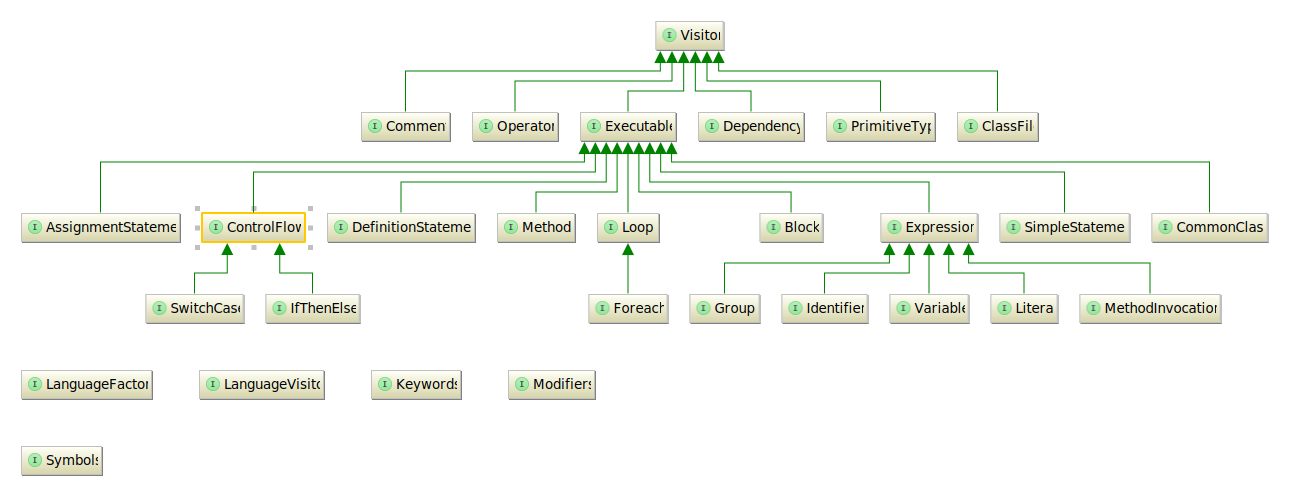
\includegraphics[width=0.6\textwidth]{resources/languagemodel_common}
    \end{center}
    \caption{UML Klassendiagramm des Zielsprachenmodells}
    \label{fig:language_model}
\end{figure}

Die Aufgabe des Generators ist die Transformierung des Applikationsmodells in das Modell der Zielsprache. Um die gewünschte Austauschbarkeit der Zielsprache zu gewährleisten wurde ein Sprachenmodell entworfen welches allgemeine Elemente einer Objektorientierten Programmiersprache enthält. %Anforderungen erstellen und referenzieren.

\subsection{Language Visitor}
\label{sec:language_visitor}

Kapitel gehört eher zu Generator

\subsection{PHP-Zielsprachenmodell}
\label{sec:php_target_language_model}

% Sprachschnittstelle!
\subsection{Language Factory}
\label{sec:language_factory}

Um eine Zielsprachenunabhänhigkeit zu erreichen, wird dem Generator bei der Erzeugung eine \enquote{Language Factory} übergeben. Der Generator erzeugt Sprachelemente nur über diese Factory. Ein Aufruf einer Factorymethode gibt ein Element der vom Typ der Sprache zurück, der Generator kennt aber nur den Interface-Typ. Für ihn ist die konkrete Implementierung somit transparent.
